\documentclass[nonatbib,numbers,10pt]{llncs}

\usepackage{fontspec}
\setmainfont{Liberation Sans}
\usepackage{subfigure}


% Geometry
\usepackage{geometry}
\geometry{
	a4paper,
	total={170mm,257mm},
	top=4.5cm,
	right=4cm,
	bottom=6.5cm,
	left=5cm,
}

\usepackage{epigraph}
% Math
\usepackage{amsmath}
\usepackage{amssymb}
\usepackage{stmaryrd}
% Code listing
\usepackage{minted}
%\usemintedstyle{friendly}
\usemintedstyle{tango}
\usepackage{algorithm}
\usepackage[noend]{algpseudocode}
% Colors
\usepackage{xcolor, color, colortbl}
\colorlet{CodeBg}{gray!90}
\usepackage{color, colortbl}
\definecolor{Gray}{rgb}{0.9,0.9,0.9}
\definecolor{bblue}{HTML}{1D577A}
\definecolor{rred}{HTML}{C03425}
\definecolor{ggreen}{HTML}{8BB523}
\definecolor{ppurple}{HTML}{6B1B7F}
\definecolor{pblack}{HTML}{000000}
\definecolor{pyellow}{HTML}{C0B225}
% Links
\usepackage{hyperref}
\definecolor{linkcolour}{rgb}{0,0.2,0.6}
\hypersetup{colorlinks,breaklinks,urlcolor=linkcolour,linkcolor=linkcolour,citecolor=linkcolour}
% Graphs
\usepackage{tikz}
\usetikzlibrary{calc}
\usetikzlibrary{trees}
\usetikzlibrary{positioning}
\usepackage{pgfplots}
% Graphics
\usepackage{graphics}
\graphicspath{{figures/}} % Location of the graphics files

\newcommand\todo[1]{\textcolor{red}{#1}}
\newcommand{\w}[1]{\textit{"#1"}}
\newcommand\s{\textsc}

\newcommand{\Order}[5]{
	\[
	\mathcal{#1}_{#5}\llbracket #2 \leftarrow #3 \mid \{ #4 \} \rrbracket.
	\]
}
\newcommand{\Orderr}[5]{
	\mathcal{#1}_{#5}\llbracket #2 \leftarrow #3 \mid \{ #4 \} \rrbracket.
}
\newcommand{\Orderrr}[5]{
	\mathcal{#1}_{#5}\llbracket #2 \leftarrow #3 \mid \{ #4 \} \rrbracket
}
\newcommand{\Ord}[4]{\Order{O}{#1}{#2}{#3}{#4}}
\newcommand{\Or}[4]{\Orderr{O}{#1}{#2}{#3}{#4}}
\newcommand{\Orr}[4]{\Orderrr{O}{#1}{#2}{#3}{#4}}
\newcommand{\Con}[4]{\Order{C}{#1}{#2}{#3}{#4}}

\title{$D^3$ as a 2-MCFL}
\author{}
\institute{}

\begin{document}
\maketitle

\begin{abstract}
We discuss the open problem of parsing the Dyck language of 3 symbols, $D^3$, using a 2-Multiple Context-Free Grammar. We tackle this problem by implementing a number of novel techniques and present the associated software packages we developed.
\end{abstract}

\keywords{Dyck Language; multiple context free grammars (MCFG)}


\section{Introduction}\label{sec1}
Our goal with this paper is the analysis of the 3-dimensional Dyck language, $D^3$, under the scope of a 2-multiple context-free language, 2-MCFL. For brevity's sake, this chapter only serves as a brief introductory guide towards relevant papers, where the interested reader will find definitions, properties and various correspondences of the problem. 

$D^3$ is defined over a lexicographically ordered alphabet ($a$, $b$, $c$) as the generalized language of well-balanced parentheses\cite{moortgat}. It is a subset of MIX\cite{kanazawa}, which has already been proven expressible by a 2-MCFG\cite{salvati}; the class of multiple context-free grammars that operate on pairs of strings\cite{gotzmann}. 

There are a number of interesting correspondences to $D^3$. Firstly, a word of $D^3$ can be presented as a \textit{standard Young Tableau}, which is a rectangular table with strictly ascending rows/columns containing as entries the numbers $\{1,2,\dots,n\}$ where $n$ the  total number of symbols in the word. The Young Tableau can be obtained by placing (in order) each character's index to the row corresponding to its lexicographical ordering (e.g. an $a$ is placed on the first row)\cite{moortgat}. 

Another correspondence exists between $D^3$ and combinatorial \textit{Spider Webs}, a special category of directed planar graphs embedded on a disk\cite{petersen}. Spider Webs can be obtained through the application of a set of rules, known as the \textit{Growth Algorithm}, which operates on pairs of neighbouring nodes, collapsing them into a singular intermediate node, transforming them into a new pair or eliminating them altogether. At termination, this process produces a well-formed Spider Web, which, in the context of $D^3$, can be interpreted as a visual representation of parsing a word.

A bijection links Young Tableaux with Spider Webs. Specifically, the \textit{Jeu-de-taquin} algorithm can be applied on a Young Tableau, which transforms it to another one through an act called \textit{promotion}. Subsequent promotions will eventually result in the initial tableau. Promotion thus defines an equivalence class, which we call an \textit{orbit}\cite{petersen}.

\section{Modeling Techniques}\label{sec2}
We now present a number of novel techniques that we developed as an attempt to solve the problem at hand, incrementally moving towards more complex and abstract grammars. For the purpose of experimentation we have implemented these techniques, based on a software library for parsing MCFGs\cite{ljunglof}. The resulting Python code is open-source and available online\footnote{\url{https://github.com/omelkonian/dyck}}.

\subsection{Triple Insertion}
To set things off, we start with the grammar of \textit{triple insertion}. This grammar operates on non-terminals $\s{W}(x,y)$, producing $\s{W}(x',y')$ with an additional triplet \textit{a, b, c} that respects the partial orders $x<y$ and $a<b<c$. The end-word is produced through the concatenation of $(x,y)$.

\begin{figure}
  \begin{minipage}{0.45\textwidth}
  	\centering
    \begin{align}
	\setcounter{equation}{0}
	\s{S}(xy) \leftarrow \s{W}(x,y)&. \\
	\s{W}(\epsilon, xy\textbf{abc}) \leftarrow \s{W}(x,y)&. \\
	... \nonumber \\
	\setcounter{equation}{60}
	\s{W}(\textbf{abc}xy, \epsilon) \leftarrow \s{W}(x,y)&. \\
	\s{W}(\epsilon, \textbf{abc})&. \\
	... \nonumber \\
	\setcounter{equation}{64}
	\s{W}(\textbf{abc}, \epsilon)&.
	\end{align}
	\caption{Grammar of triple insertions}
    \label{fig:1}
  \end{minipage} \hspace{0.05\textwidth}
  \begin{minipage}{0.55\textwidth}
  	\centering
  	\begin{align*}
	&\s{S}(xy) \leftarrow \s{W}(x,y). \\
	&\Or{\s{W}}{\epsilon}{a < b < c}{2} \\
	&\Or{\s{W}}{\s{W}}{x < y,\ a < b < c}{2}
	\end{align*}
	\caption{$\mathcal{G}_0$: Meta-grammar of triple insertions}
	\label{fig:meta-ins}
  \end{minipage}
\end{figure}

Despite being conceptually simple, this grammar consists of a large number of rules. Its expressivity is also limited; the prominent weak point is its inability to manage the effect of \textit{straddling}, namely the generation of words whose substituents display complex interleaving patterns. Refer to Fig.\ref{fig:fmp} for an example.
\subsection{Meta-Grammars}
To address the issue of rule size, we introduce the notion of \textit{meta-grammars}, loosely inspired by Van Wijngaarden's work\cite{vanwijn}, which allows a more abstract view of the grammar as a whole. Specifically, we define $\mathcal{O}$ as the \textit{meta-rule} which, given a rule format, a set of partial orders (over the tuple indices of its premises and/or newly added terminal symbols), and the MCFG dimensionality, automatically generates all the order-respecting permutations. An example of how we can abstract away from explicitly enumerating the entirety of our initial rules is showcased in Fig. \ref{fig:meta-ins}.

This approach enhances the potential expressivity of our grammars as well. For instance, we can now extend the previous with a single meta-rule that allows two non-terminals $\s{W}(x,y)$, $\s{W}(z,w)$ to interleave with one another, producing rearranged tuple concatenations and allowing some degree of straddling to be generated:
\[
\mathcal{G}_1: \mathcal{G}_0 + \Or{\s{W}}{\s{W}, \s{W}}{x < y,\ z < w}{2}
\]

The addition of this rule gets us closer to completeness, but we are still not quite there. We have thus far only used a single non-terminal, not utilizing the expressivity that an MCFG allows. To that end, we propose non-terminals to represent incomplete word \textit{states}; that is, words that either have an extra symbol or miss one. The former are \textit{positive} states, whereas the latter are \textit{negative}. The inclusion of these extra states would allow for more intricate interactions. Interestingly, there is a direct correspondence between these non-terminals and the nodes of Petersen's growth algorithm.

This meta-grammar, given below, consists of base cases for positive states, possible state interactions, closures of pairs of inverse polarity and a universally quantified meta-rule that allows the combination of any incomplete state with a well-formed one (i.e. non-terminal $\s{W}$).
\begin{figure}
    \centering
    \begin{subfigure}{}
		\begin{minipage}{.2\textwidth}
		\begin{align*}
		&\s{S}(xy) \leftarrow \s{W}(x,y). \\
		&\Or{\s{W}}{\epsilon}{a < b < c}{2} \\
		&\Or{\s{A}^+}{\epsilon}{a}{2} \\
		&\Or{\s{B}^+}{\epsilon}{b}{2} \\
		&\Or{\s{C}^+}{\epsilon}{c}{2} \\
		&\Or{C^-}{A^+, B^+}{x < y < z < w}{2} \\
		&\Or{B^-}{A^+, C^+}{x < y < z < w}{2}
		\end{align*}
		\end{minipage}
	\end{subfigure}%
	~ ~ ~
    \begin{subfigure}{}
	    \begin{minipage}{.2\textwidth}
		\begin{align*}
		&\Or{A^-}{B^+, C^+}{x < y < z < w}{2} \\
		&\Or{A^+}{C^-, B^-}{x < y < z < w}{2} \\
		&\Or{B^+}{C^-, A^-}{x < y < z < w}{2} \\
		&\Or{C^+}{B^-, A^-}{x < y < z < w}{2} \\
		&\Or{W}{A^+, A^-}{x < y < z < w}{2} \\
		&\Or{W}{C^-, C^+}{x < y < z < w}{2} \\
		&\forall \ \s{K} \in \{\textsc{A}^{+/-},\ \textsc{B}^{+/-},\ \textsc{C}^{+/-}\}:\\ 
		&\quad\Or{\s{K}}{\s{K}, \s{W}}{x < y,\ z < w}{2}
		\end{align*}
		\end{minipage}
   \end{subfigure}
    \caption{$\mathcal{G}_2$: Meta-grammar of incomplete states}%
    \label{fig:example}
\end{figure}

A further extension can be achieved through universally quantifying the notion of triple insertion, which is unique in the sense that it can insert three different terminals, each at a different position:
\[
\mathcal{G}_3: \mathcal{G}_2 + \forall \ \s{K} \in \{\textsc{A}^{+/-},\ \textsc{B}^{+/-},\ \textsc{C}^{+/-}\}: \Or{\s{K}}{\s{K}}{x < y,\ a < b < c}{2}
\]

\subsection{Rule Inference}\label{aris}	
The improved performance of the above approaches again proved insufficient to completely parse $D^3$. Our meta-rules are over-constrained by imposing a total order on the tuple elements, due to their inability to keep track of where the extra character(s) is. To overcome this, we split each state into multiple position-aware, \textit{refined} states. Doing so revealed a vast amount of new interactions, as evidenced by the below alteration to the original $\s{A}^+$, $\s{B}^+$ interaction (where $y$ can now occur after $z$ or $w$):
\[
\Or{C^-}{A^+_{left}, B^+}{x < y, x < z < w}{2}
\]

In order to accommodate the interactions between this increased number of states, we need to keep track of both internal and external order constraints. At this point, the abstraction offered by our meta-grammar approach does not cover our needs any more. The same difficulty that we had encountered before is prominent once more, except now at an even higher level. 

As a solution to the aforementioned limitation, we propose a system that can automatically create a full-blown m-MCFG given only the states it consists of. To accomplish this, we assign each state a unique \textit{descriptor} that specifies the content of its tuple's elements. Aligning these descriptors with the tuple, we can then infer the descriptor of the resulting tuple of every possible state interaction. For the subset of those interactions whose resulting descriptor is matched with a state, we can now automatically infer the rule.

Formally, the system is initialized with a map $\mathcal{D}$, whose domain, $dom(\mathcal{D})$, is a set of \textit{state identifiers} and its codomain, $codom(\mathcal{D})$, is the set of their corresponding \textit{state descriptors} as illustrated in Fig.\ref{fig:desc}.

\vspace{-10pt}
\hspace{-16pt}
\begin{minipage}{.22\textwidth}
\begin{figure}[H]
\begin{align*}
\s{W} &\mapsto (\epsilon, \epsilon) \\
\s{A}^+_{l} &\mapsto (a, \epsilon) \\
\s{A}^+_{r} &\mapsto (\epsilon, a) \\
\s{B}^+_{l} &\mapsto (b, \epsilon)\\
&... \\
\s{B}^-_{l, r} &\mapsto (a, c) \\
\s{C}^-_{l} &\mapsto (ab, \epsilon) \\
\s{C}^-_{r} &\mapsto (\epsilon, ab) \\
\s{C}^-_{l, r} &\mapsto (a, b)
\end{align*}
\caption{Map $\mathcal{D}$}
\label{fig:desc}
\end{figure}
\end{minipage}
\hspace{0.08\textwidth}
\begin{minipage}{.68\textwidth}
\begin{algorithm}[H]
\caption{ARIS: Automatic Rule Inference System}\label{euclid}
\begin{algorithmic}
\Procedure{aris}{$\mathcal{D}$}
	\For{$X \mapsto (d_1,\dots ,d_n) \in \mathcal{D}$}
		\State \textbf{yield} $X(d_1,\dots,d_n).$
	\EndFor
	\For{$X,Y \in dom(\mathcal{D})^2$}
		\State $(X_{ord},\ Y_{ord}) \leftarrow (x<y<\dots,\ z<w<\dots)$ 
		\For{$(d_1,...,d_n) \in \Orr{\_}{X,Y}{X_{ord}, Y_{ord}}{2}$}
			\For{$S' \in \textsc{eliminate}((d_1,\dots ,d_n), \mathcal{D})$}
				\State \textbf{yield} $S'(d_1,\dots ,d_n) \leftarrow X, Y.$
			\EndFor
		\EndFor
	\EndFor
\EndProcedure
\\
\Procedure{eliminate}{$(d_1,\dots ,d_n), \mathcal{D}$}
	\For{$matches \in \textsc{all\_abc\_triplets}(d_1,\dots ,d_n)$}
		\For{$i \in 0\dots n/3$}
			\For{$S' \in \textsc{remove\_abc\_triplets}(matches, i)$}
				\If {$S' \in codom(\mathcal{D})$}
					\State \textbf{yield} $S'$
				\EndIf				
			\EndFor
		\EndFor
	\EndFor
\EndProcedure
\end{algorithmic}
\end{algorithm}
\end{minipage}

\vspace{10pt}
Meta-grammars accelerated the process of creating grammars, by letting us simply describe rules instead of explicitly defining them. ARIS builds upon this notion to raise the level of abstraction even further; one needs only specify a grammar's states and its descriptors, thus eliminating the need to define rules or even meta-rules.

\section{Tools \& Results}
\subsection{Grammar Utilities}
We have implemented the modelling techniques described in section \ref{sec2} and distributed a Python package, called \textbf{dyck}, which provides the programmer with a \textit{domain-specific language} close to this paper's mathematical notation. To facilitate experimentation, our package includes features such as grammar selection, time measurements, word generation and soundness/completeness checking. The following example demonstrates the definition of $\mathcal{G}_1$:

\begin{center}
\begin{minipage}{0.5\textwidth}
\begin{minted}[baselinestretch=1.1, fontsize=\small]{python}
from dyck import *
G_1 = Grammar([
    ('S <- W', {(x, y)}),
    O('W', {(a, b, c)}),
    O('W <- W', {(x, y), (a, b, c)}),
    O('W <- W, W', {(x, y), (z, w)}) 
])
\end{minted}
\end{minipage}
\end{center}


\subsection{Visualization}
As counter-examples began to grow in size and number, we realised the necessity of a visualization tool to assist us in identifying properties they may exhibit. To that end, we distribute another Python package, called \textbf{dyckviz}, which allows the simultaneous visualization of tableau-promotion and web-rotation (grouped in their corresponding equivalence classes). An example of a web as rendered by our tool is given in Fig.\ref{fig:web}.

Young tableaux in an orbit are colour-grouped by their column indices, which sheds some light on how the \textit{jeu-de-taquin} actually influences the structure of the corresponding Dyck words. Interesting patterns have began to emerge, which still remain to be properly investigated. 


\begin{figure}
\begin{center}
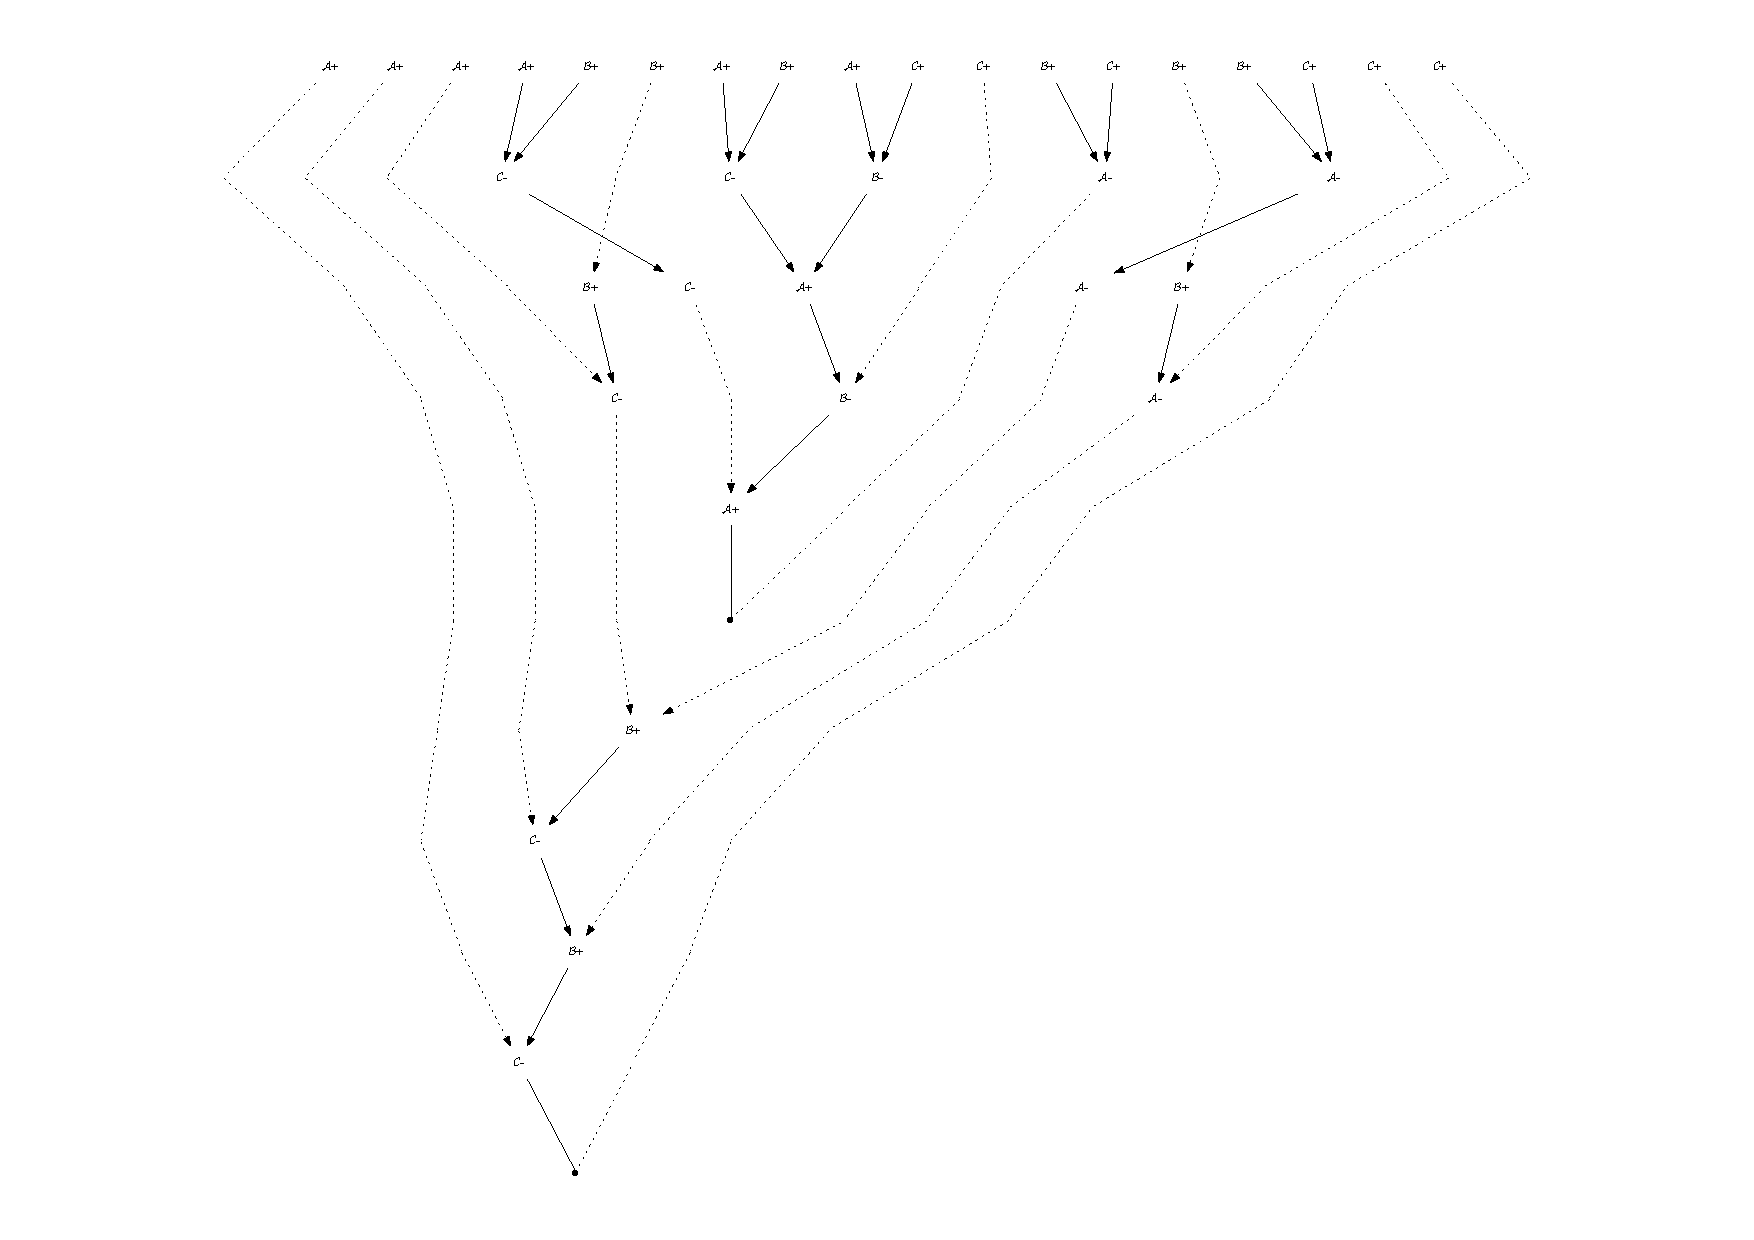
\includegraphics[width=0.75\textwidth]{web.pdf}
\caption{Spider web of \w{abaacbbacbabaccbcc}}
\label{fig:web}
\end{center}
\end{figure}


\subsection{Grammar Comparisons}
We display three charts, depicting the number of rules, percentage of counter-examples and computation times of each of our grammars for $D^3_n$ with $n$ ranging from $2$ to $6$ (where $n$ denotes the number of $abc$ triplets). Even though none of our proposed grammars is complete, we observe that as grammars get more abstract, the number of failing parses steadily declines. This however comes at the cost of rule size growth, which in turn is associated with an increase in computation times. What this practically means is that we are unable to continue testing more elaborate grammars or scale our results to higher orders of $n$ (note that $| \! | D^3_n | \! |$ also has a very rapid rate of expansion)\cite{moortgat}.
\begin{figure}[h]
% Rule size
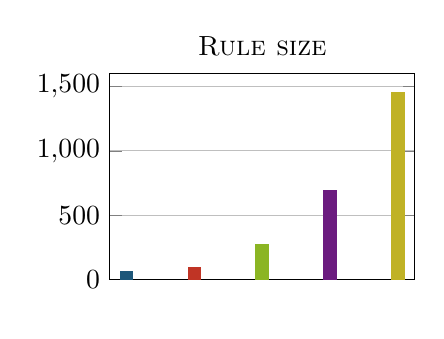
\begin{tikzpicture}
    \begin{axis}[
        width  = 0.45\textwidth,
        height = 4.2cm,
        major x tick style = transparent,
        ybar=20,
        bar width=4.5pt,
        ymajorgrids = true,
        ylabel = {\textsc{Rule size}},
        every axis x label/.style={
  			  at={(ticklabel* cs:1.05)},
  			  anchor=west,
  			  },
			every axis y label/.style={at={(current axis.north)},above=1mm},
        symbolic x coords={$ $},
        xtick = data,
        scaled y ticks = false,
        enlarge x limits=0.5,
        ymin=0,
        legend cell align=left,
        legend style={
        		at={(0.5,-0.15)},
				anchor=north,
				legend columns=-1
			},
    ]
        \addplot[style={bblue,fill=bblue,mark=none}]
            coordinates {($ $, 65)};
        \addplot[style={rred,fill=rred,mark=none}]
             coordinates {($ $,95)};
        \addplot[style={ggreen,fill=ggreen,mark=none}]
             coordinates {($ $,270)};
        \addplot[style={ppurple,fill=ppurple,mark=none}]
             coordinates {($ $,690)};
        \addplot[style={pyellow,fill=pyellow,mark=none}]
             coordinates {($ $,1456)};
    \end{axis}
\end{tikzpicture}
% Computation Time
\hspace{0.07\textwidth}
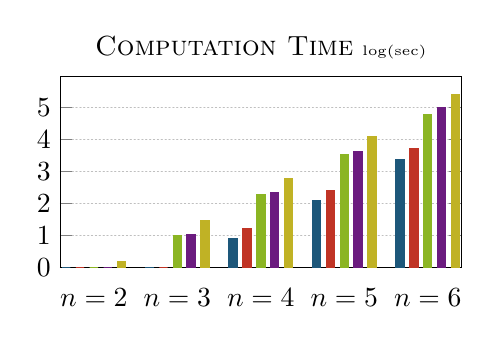
\begin{tikzpicture}
    \begin{axis}[
        width  = 0.55*\textwidth,
        height = 4cm,
        major x tick style = transparent,
        ybar=5*\pgflinewidth,
        bar width=3pt,
        ymajorgrids = true,
        ylabel = {\textsc{Computation Time} \tiny log(sec)},
        every axis x label/.style={
  			  at={(ticklabel* cs:1.05)},
  			  anchor=west,
  			  },
			every axis y label/.style={at={(current axis.north)},above=1mm},
        symbolic x coords={$n=2$,$n=3$,$n=4$,$n=5$,$n=6$},
        xtick = data,
        scaled y ticks = false,
        enlarge x limits=0.1,
        ymin=0,
        legend cell align=left,
        legend style={
        		at={(0.5,-0.25)},
				anchor=north,
				legend columns=-1
			},
		ytick={0, 1, ..., 5},
		y grid style={densely dotted, line cap=round},
    ]
		 \addplot[style={bblue,fill=bblue,mark=none}]
           coordinates {($n=2$, 0) ($n=3$,-0.3) ($n=4$,0.9) ($n=5$,2.1) ($n=6$,3.37)};           
        \addplot[style={rred,fill=rred,mark=none}]
             coordinates {($n=2$,0) ($n=3$,0) ($n=4$,1.23) ($n=5$,2.39) ($n=6$,3.73)};             
        \addplot[style={ggreen,fill=ggreen,mark=none}]
             coordinates {($n=2$,0) ($n=3$,1) ($n=4$,2.28) ($n=5$,3.54) ($n=6$,4.79)};
        \addplot[style={ppurple,fill=ppurple,mark=none}]
             coordinates {($n=2$,0) ($n=3$,1.04) ($n=4$,2.34) ($n=5$,3.64) ($n=6$,4.99)};
        \addplot[style={pyellow,fill=pyellow,mark=none}]
             coordinates {($n=2$,0.17) ($n=3$,1.46) ($n=4$,2.77) ($n=5$,4.09) ($n=6$,5.42)};
    \end{axis}
\end{tikzpicture}
% Counter-examples
\begin{center}
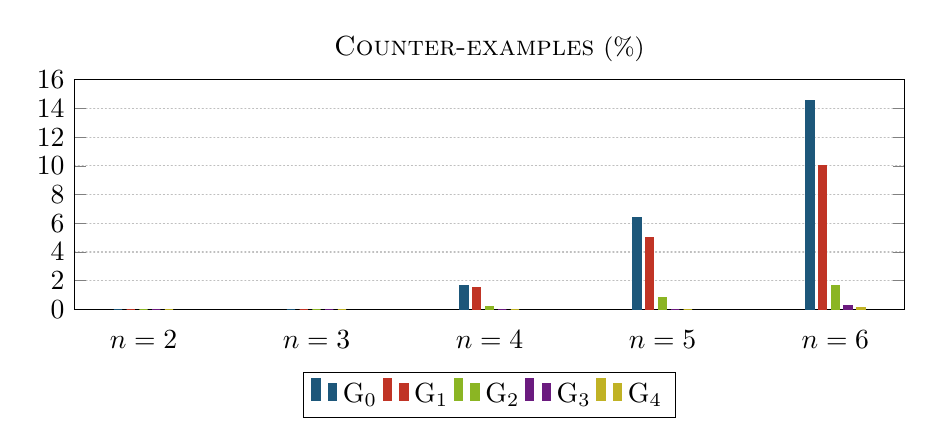
\begin{tikzpicture}
    \begin{axis}[
        width  = 1*\textwidth,
        height = 4.5cm,
        major x tick style = transparent,
        ybar=4*\pgflinewidth,
        bar width=3pt,
        ymajorgrids = true,
        ylabel = {\textsc{Counter-examples} \small (\%)},
        every axis x label/.style={
  			  at={(ticklabel* cs:1.05)},
  			  anchor=west,
  			  },
			every axis y label/.style={at={(current axis.north)},above=1mm},
        symbolic x coords={$n=2$,$n=3$,$n=4$,$n=5$,$n=6$},
        xtick = data,
        scaled y ticks = false,
        enlarge x limits=0.1,
        ymin=0,
        legend cell align=left,
        legend style={
        		at={(0.5,-0.27)},
				anchor=north,
				legend columns=-1
			},
		ytick={0, 2, ..., 17},
		y grid style={densely dotted, line cap=round},
    ]
        \addplot[style={bblue,fill=bblue,mark=none}]
            coordinates {($n=2$, 0) ($n=3$,0) ($n=4$,1.7) ($n=5$,6.42) ($n=6$,14.55)};
        \addplot[style={rred,fill=rred,mark=none}]
             coordinates {($n=2$,0) ($n=3$,0) ($n=4$,1.5) ($n=5$,5) ($n=6$,10)};
        \addplot[style={ggreen,fill=ggreen,mark=none}]
             coordinates {($n=2$,0) ($n=3$,0) ($n=4$,0.2) ($n=5$,0.8) ($n=6$,1.7)};
        \addplot[style={ppurple,fill=ppurple,mark=none}]
             coordinates {($n=2$,0) ($n=3$,0) ($n=4$,0) ($n=5$,0) ($n=6$,0.3)};
        \addplot[style={pyellow,fill=pyellow,mark=none}]
             coordinates {($n=2$,0) ($n=3$,0) ($n=4$,0) ($n=5$,0) ($n=6$,0.15)};
        \legend{G$_0$,G$_1$,G$_2$,G$_3$,G$_4$,G$_5$}
    \end{axis}
\end{tikzpicture}
\end{center}
\caption{Performance measures}
\end{figure}

\section{Road to Completeness}\label{sec4}
To our knowledge, no other attempt has come so close to modelling $D^3$ with a 2-MCFG. We attribute this to the combination of a pragmatic approach with results from existing theoretical work. In this chapter, we present a collection of additional ideas, which we consider worthy of further exploration.

\paragraph{\textbf{First-Match Policy and Relinking}}
Possibly the most intuitive way of checking whether a word $w$ is part of $D^3_n$ is checking whether a pair of links occur that match $a_i$ to $b_i$ and $b_i$ to $c_i \ \forall i \in n$. We call this process of matching the \textit{first-match policy}. The question arises whether a grammar can accomplish inserting a triplet of $a$, $b$, $c$, that would abide by the first-match policy. If that were the case, it would be relatively easy to generalize this ability by induction to every $n \in \mathbb{N}$. Unfortunately, the answer is seemingly negative; the expressiveness provided by a 2-MCFG does not allow for the arbitrary insertions required. On a related note, being able to produce a word state $W(x,y)$ where $w=xy$ and $x$ any possible prefix of $w$, gives no guarantee of being able to produce the same word with an extra triplet inserted due to the straddling property. 

However, if rules existed that would allow for match-making and breaking, i.e. match \textit{relinking}, an inserted symbol could be temporarily matched with what might be its first match-policy in a local scope, and then relink it to its correct match when merging two words together.
\begin{figure}[h!]
\centering

\begin{tikzpicture}[every node/.style={anchor=base},xscale=.25,yscale=.4]
\node (n0) at (0,0) {$a$};
\node (n1) at (1,0) {$b$};
\node (n2) at (2,0) {$a$};
\node (n3) at (3,0) {$b$};
\node (n4) at (4,0) {$a$};
\node (n5) at (5,0) {$c$};
\node (n6) at (6,0) {$b$};
\node (n7) at (7,0) {$c$};
\node (n8) at (8,0) {$a$};
\node (n9) at (9,0) {$b$};
\node (n10) at (10,0) {$c$};
\node (n11) at (11,0) {$c$};
\draw (n0) edge [rred, bend left=90] (n1);
\draw (n1) edge [rred, bend right=90] (n5);
\draw (n2) edge [ggreen, bend left=90] (n3);
\draw (n3) edge [ggreen, bend right=90] (n7);
\draw (n4) edge [bblue, bend left=90] (n6);
\draw (n6) edge [bblue, bend right=90] (n10);
\draw (n8) edge [pyellow, bend left=90] (n9);
\draw (n9) edge [pyellow, bend right=90] (n11);
\end{tikzpicture}
\caption{First-match policy for \w{ababacbcabcc}}
\label{fig:fmp}
\end{figure}
\paragraph{\textbf{Growth Rules}}
Although $\mathcal{G}_2$ comes close to realizing the growth algorithm, not all of the growth rules can be translated into a 2-MCFG setting. It would be an interesting endeavour to attempt to model the element-swapping behaviour of these rules that produce two output states, without resorting to more expressive formalisms (e.g. context-sensitive grammars).
\paragraph{\textbf{Insights from promotion}}
An interesting question is whether promotion can be handled by a 2-MCFG (as a \textit{context-free rewriting system}). If so, it could be worth looking into the properties of orbits, to test for instance if there are promotions within an orbit that can be easier to solve than others. Solving a single promotion and transducing the solution to all equivalent words could then be a guideline towards completeness. 

\section{Conclusion}
We tried to accurately present the intricacies of $D^3$ and the difficulties that arise when attempting to model it under the scope of a 2-MCFL. We have developed and introduced some novel techniques and tools, which we believe can be of use even outside the problem's narrow domain. We have largely expanded on the existing tools to accommodate MIX-style languages and systems of meta-grammars in general.

Despite our best efforts, the question of whether $D^3$ can actually be encapsulated within a 2-MCFG still remains unanswered. Regardless, this problem has been very rewarding to pursue, and we hope to have intrigued the interested reader enough to further research the subject, use our code, or strive for a solution on his/her own.

\bibliographystyle{splncs03}
\bibliography{sources}

\end{document}
